\documentclass{fpgairpods}
\usepackage[letterpaper, margin=1in]{geometry}

\addbibresource{report.bib}
\graphicspath{{figs/}}

\setlist{noitemsep, topsep=0pt}

\begin{document}

\title{\textit{FPGAirPods}: Implementing Active Noise Cancellation on a Xilinx Artix-7 FPGA}
\date{6.111 Introductory Digital Systems Laboratory \\ \textit{Massachusetts Institute of Technology} \\ \today}
\author{Ben Kettle \\ \ttt{bkettle@mit.edu} 
\and Nicholas Ramirez \\ \ttt{ramirezn@mit.edu} \and Gokul Kolady \\ \ttt{gokulk@mit.edu}}

\maketitle
\tableofcontents
\listoffigures

\newpage
\section{Introduction and Motivation}

Noise cancellation is clearly in demand---at the time of writing this, Apple has just released AirPods Max for \$550, and active noise cancellation can be found everywhere from air ducts to cars. However, it's often treated as a black box---our team was interested in looking inside this black box to learn about the intricacies of implementing active noise cancellation on a real system. Further, we were all interested in audio processing and hoped to take advantage of the FPGA's ability to perform operations quickly and in parallel for our 6.111 final project.

Implementing active noise cancellation as seen in over-ear and in-ear headphones such as the Bose QC35 and the AirPods Pro (our project's namesame), then, seemed like a great choice that would allow us to combine all these interests.

We knew going into the project that it would be difficult, and one of the things that made it particularly difficult would be the need for solid test hardware and reliance on that hardware to achieve any form of functionality. Indeed, this proved to be the case, and we ran into several difficulties along the way, as we will describe in this report. Despite these difficulties, we learned more than we could've hoped about the importance of defining modules clearly, testbenching to avoid wasting long compile time, and more, in the end building an end result that we are proud of.

\section{Project Overview} % talk about how the system works right now, here is where we should put graphs of cancellation effectiveness at different frequencies
% I think we can generate those graphs by making a python script to analyze ILA output and give the average amplitude of the wave, then we just compare these to find a dB cancelled
% block diagram goes with this. Talk about general idea about functionality
After a significant amount of research and after communicating with course staff about possibilities, we decided to base our system around the Least Mean Squares algorithm for replicating an unknown system. In our case, this unknown system was the system that would create a signal that cancels the ambient noise for our model of a headphone. We would model this system using a Finite Impulse Response (FIR) filter, and we would use the LMS algorithm to determine the coefficients that brought the output of this model system as close as possible to the optimal anti-noise signal.

For our test system, we decided on an ambient noise microphone, a speaker to output the calculated anti-noise signal, and a feedback microphone to measure the effectiveness of this anti-noise signal, as described in greater detail in the next section. Once we had signals from these microphones, our goal was to process the signal from the ambient noise microphone and, in the time it takes for the sound wave to travel from the ambient microphone to the time it crosses the speaker, calculate the correct signal to output from the speaker in order to cancel out as much of the incoming noise as possible.

In effect, this meant that our FIR filter would be characterizing the frequency response of our full system, including the enclosure and the speaker itself, as well as the delay that existed between our ambient microphone and our speaker. In theory, the LMS algorithm should determine different scaling factors for each incoming frequency depending on the way that our system responded to those incoming frequencies, and the FIR should them apply these scaling factors to the incoming signal in order to calculate the next output.

The FPGA itself handles the computational side of the active noise cancellation. The general flow of the system starts with sampling the incoming signal from the microphones, processing the samples, and outputting the anti-noise signal. We decided on a sampling rate of 65 kHz as it is the maximum sampling rate supported by the microphones. In terms of logistics for the FPGA timing, we based our target latency on the time it takes for a sound signal to travel from the ambient microphone to the speaker. Since the ambient microphone is about 2 cm away from the speaker and sound travels around 343 meters per second, we have around 5830 clock cycles to make all of our computations and output an anti-noise signal. In figure \ref{fig:systemlatency}, we can see that our final system latency was well within this bound, taking around 130 clock cycles output anti-noise for a sample after initially receiving it.

\begin{figure}
\centering
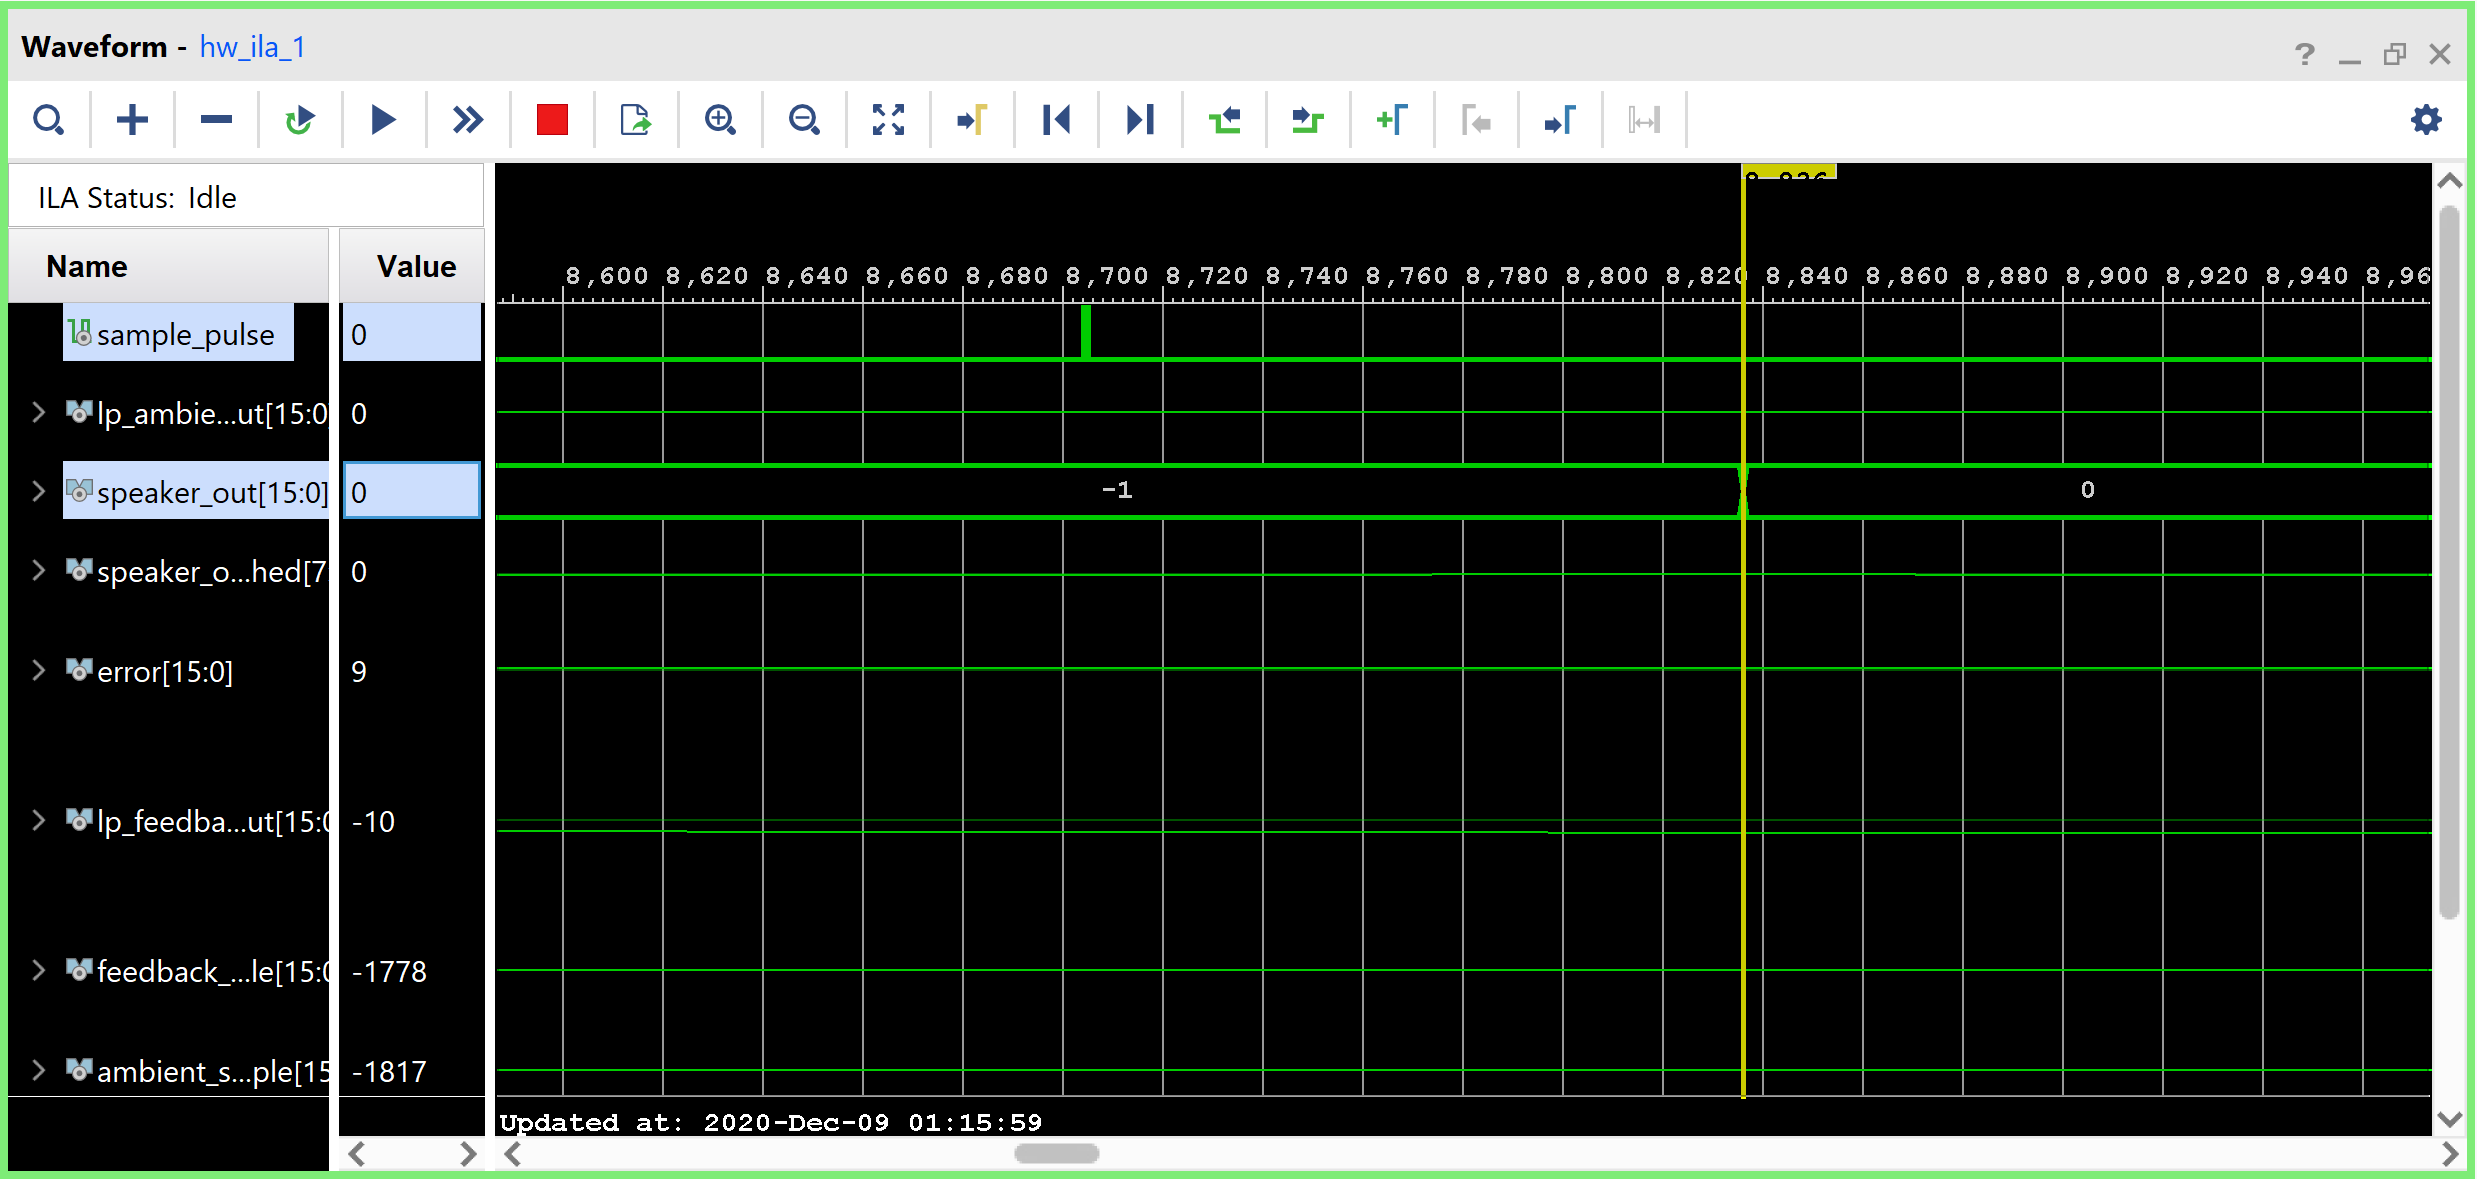
\includegraphics[width=300pt]{./figs/system_latency_ila.png}
\caption{System latency (clock cycles necessary to process a sample and output anti-noise)}
\label{fig:systemlatency}
\end{figure}

For processing the samples, we used the Normalized Least Mean Squares (NLMS) adaptive filter to continually calculate coefficients that aim to minimize the error function --- i.e., the noise that makes it through and is not cancelled out. These updated coefficients are then applied to the input ambient sample by a Finite Impulse Response (FIR) filter and played out the speaker to cancel the noise. 

This proved to be very difficult. Our target goal at the beginning of the project was to be able to cancel ambient noise effectively, but in its current state, our system is unable to effectively create an anti-noise signal that works for ambient noise. However, we were able to achieve our base goal of cancelling sine tones, and our system does this very effectively. Once a sine tone begins playing and is picked up by the ambient and feedback microphones, our system's NLMS algorithm is able to converge on an effective set of coefficients, typically in less than a second, and is then able to continuously cancel the incoming frequency. It can also identify when its coefficients are no longer effective, for example if the frequency of this sine tone changes, and begin searching for new coefficients that provide more effective cancellation. In order to quantify this performance, we measured the amplitude of the signal received by the feedback microphone while playing sine tones of various frequencies, with our anti-noise signal both on and off. We then converted took the ratio into decibels for easy comparison by taking $20\log{\frac{\text{on}}{\text{off}}}$. The result of this analysis can be seen in figure \ref{chart:anc_freq_response}---at the frequencies our system cancelled most effectively, around 400Hz, we achieved 30dB of cancellation between when ANC is turned off and when ANC is turned on.
% we did not achieve our goal of ambient noise cancellation. However, we achieved effective single-frequency sine tone cancellation. Graphs 


\begin{figure}
    \centering
    \begin{tikzpicture}
        \begin{axis}[
            title={Effect of FPGAirPods ANC on Ambient Sine Tones},
            xlabel={External Frequency Played (Hz)}, 
            ylabel={Cancellation by ANC (dB)}
        ]
        \addplot table [
                x=f, 
                y=db, 
                col sep=comma, 
                scatter, 
                only marks 
            ] {charts/frequency_cancellation.csv};
        \end{axis}
    \end{tikzpicture}
    \caption{Difference between feedback signal received with ANC on and with ANC off}
    \label{chart:anc_freq_response}
\end{figure}

\begin{sidewaysfigure}
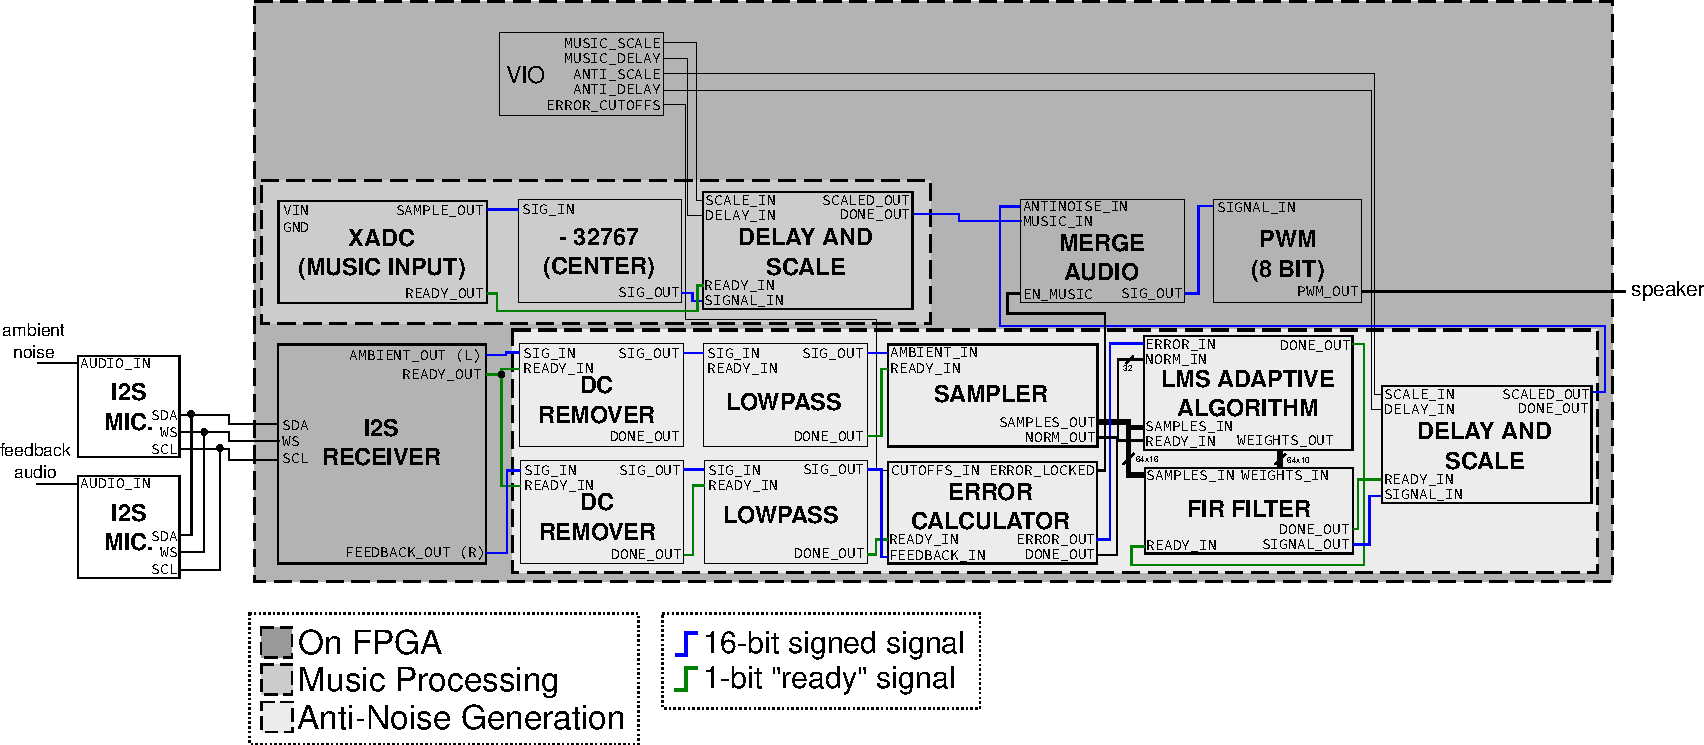
\includegraphics[width=\textheight]{./figs/block_diagram.pdf}
\caption{The high-level block diagram for our system.}
\label{fig:blockdiagram}
\end{sidewaysfigure}

\newpage
\section{Hardware Testing Setup}
\subsection{Testing Hardware (Ben)}
In order to demonstrate that our system was functional, a system to test on was crucial. From our initial research and communicating with the course staff, we found that most existing Active Noise Cancellation (ANC) implementations use a feedback microphone to measure the result of the (hopefully destructive) interference between the speaker's anti-noise signal and the incoming ambient noise. This was especially useful for our project, as we could use this microphone to measure the performance of our system. In order to calculate the anti-noise signal to be outputted from the speaker, however, we needed a microphone that would receive sounds before they crossed the speaker. We call this the ambient noise microphone. The final crucial peripheral was the speaker itself, which was needed to output the anti-noise signal. 

We chose to use digital microphones that communicate over I2S in our system. Using a digital protocol would ensure that noise from the environment is not picked up as the signal is transmitted from the microphone to the FPGA over wires, and it would remove the need for an additional ADC for each microphone. As discussed in detail below, this required implementing an I2S receiver module to communicate with the microphones. We had to take special care when mounting these microphones---the are clearly susceptible to vibrations, and we had to be sure that any vibrations created by the speaker or the environment would not affect the readings of the microphones. To handle this, we mounted the microphones onto the inner enclosure using foam mounts that isolated the microphones from the any vibrations in the rest of our system. Another important piece was keeping the relative distances between the ambient microphone and the feedback microphone consistent---a crucial aspect of finding the anti-noise signal is accounting for the time it takes for sound waves to travel between the ambient microphone and the speaker in order to match the anti-noise signal's phase with that of the ambient noise. One advantage of using the NLMS algorithm is that some variation is tolerated here, as the FIR is capable of encoding delay. However, if this distance changes, the coefficients that were calculated previously will no longer be valid, so we needed to keep this distance as consistent as possible. The foam mounts that we created account for this as well, holding the microphones securely in place. 

For our speaker, we chose to use a consumer portable speaker in order to reduce hardware complexity. This speaker had a built in amplifier, which allowed us to drive it using the Nexys4-DDR's onboard headphone jack and DAC without need for additional electronics. One disadvantage of this, however, was that another variable was added in the controls on the speaker itself. Specifically, the speaker was battery-powered, and had a stateful volume control. This presented two challenges---we had to ensure that the charge level of the speaker was consistent and that the volume was consistent across our trials in order to isolate changes to our HDL implementation. To standardize our testing setup, we made sure to always keep the speaker plugged in to a USB port to ensure it was at full charge, and made sure that we turned the volume all the way down before turning it up 7 clicks to standardize the volume. % talk about difficulty with digital volume control, standardizing the volume that the speaker played at in order to allow full use of our coefficient resolution, as well as mounting the speaker to be in line with the microphones and to be able to charge it and give the signal without difficulty

Besides electronic peripherals, our testing system included several other materials. We identified the need for passive cancellation early on, both to ensure that the difference caused by our ANC implementation is audible, and to prevent the speaker output from reaching the ambient noise microphone causing a feedback loop. In our initial design, we had planned for only the inner container seen in Figure \ref{fig:peripherals}. However, we found that this system was far too susceptible to feedback loops, and that any deviation from the anti-noise signal by the speaker would cause the system to fail.

Further, in contrast to commercial ANC implementations that are able to have finely tuned and compact mechanical designs, our prototype was far from small. A crucial piece of the theory behind ANC is that ANC is possible only if the anti-noise source (the speaker) is located very close to the noise source---we saw an example of this in ANC from within air ducts---or very close to the receiver---this is the model that headphones with ANC use, and indeed that we were hoping to implement as well. This requirement is caused by the fact that it is only possible to accurately anticipate noise signals that are parallel to the axis of the system---if a sound is coming from an angle, the system will be unable to anticipate the wave's behavior when it crosses the speaker and when it reaches the receiver (ear). This is because without additional microphones, the system does not have enough information to determine the angle from which a wave is approaching. Given both of these issues, we iterated on our design for the enclosure itself, adding additional passive cancellation in the form of the outer foam-lined box seen in Figure \ref{fig:peripherals}. From this box, we cut out a port at the back of our inner enclosure to allow sound waves in line with the axis of our speaker to enter our system, but prevent those at other angles. This allowed us to emulate the benefits of the small form factor of commercial ANC headphones without precision machining and fabrication techniques, and prevented the output of the speaker from reaching the ambient noise microphone. In order to quantify this passive cancellation, we played a series of tones and compared the amplitudes of the ambient and feedback microphones. The amount of cancellation from ambient to feedback microphone that this analysis showed can be seen in figure \ref{chart:passive_response}.

\begin{figure}
\centering
\includegraphics[width=\textwidth]{./figs/enclosure_photos.png}
\caption{Images of testing hardware}
\label{fig:systempics}
\end{figure}

% graph of passive cancellation of various frequencies? Compare ambient and feedback mic with NC off, we will have to take these samples anyway

\begin{figure}
    \centering
    \begin{tikzpicture}
        \begin{axis}[
            title={Passive cancellation of FPGAirPods enclosure},
            xlabel={External Frequency Played (Hz)}, 
            ylabel={Cancellation (dB)}
        ]
        \addplot table [
                x=f, 
                y=db, 
                col sep=comma, 
                scatter, 
                only marks 
            ] {charts/passive_response.csv};
        \end{axis}
    \end{tikzpicture}
    \caption{Difference between ambient and feedback signals with ANC off}
    \label{chart:passive_response}
\end{figure}

\subsection{Music Playing Hardware (Ben)}
In order to enable us to play music  through the speaker as well as the anti-noise signal, we needed some way to input music into the system. To do this, we used a 3.5mm headphone jack breakout board as well as a small amount of circuitry to center the signal around 0.5V in order to make it compatible with the ADC's 0-1V range.

\begin{figure}
\centering
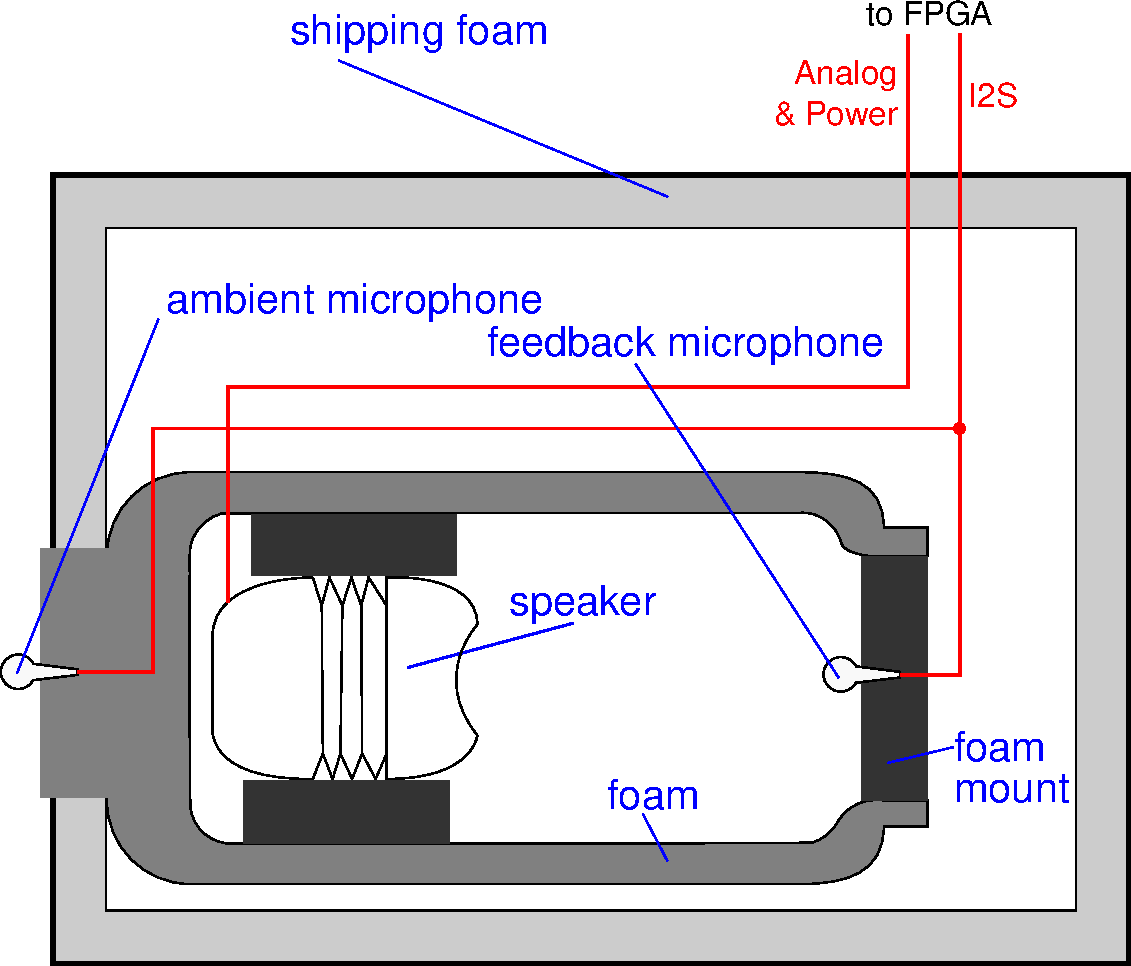
\includegraphics[width=450pt]{./figs/system_diagram_with_text.pdf}
\caption{The peripherals that will be included in our project}
\label{fig:peripherals}
\end{figure}

\section{Implementation Details}
Our implementation was structured as a series of modules each applying some processing on the incoming ambient noise signal. We devised a common scheme for all these modules to share, where in addition to any other samples or signals it requires, each module includes a \ttt{ready_in} signal and outputs a \ttt{ready_out} signal---each 1 clock cycle long. This allows us to chain many of these modules together, feeding \ttt{done_out} of each into \ttt{ready_in} of the next.

\subsection{I2S Receiver (Ben)}
This module is the origin of the \ttt{ready_in} pulse chain described above---it implements the I2S protocol as described in the datasheet\cite{mic_datasheet} for the microphones we use. In essence, this requires the creation of an \ttt{LRCLK} signal that controls whether the left (ambient) or right (feedback) mic will currently transmit. For every change of this clock, the corresponding microphone would begin sending a new sample. We drove this clock at the 4MHz, the maximum rate tolerated by the microphones, for a sampling rate through our system of 65 kHz.

For each time the \ttt{LRCLK} is low and high, we must receive the sample that is sent from the microphones. To do this, we simply shift bits into two 16-bit registers for each of the left and right channel, stopping after the top 16 bits are shifted in. The microphones report 18 bits of data, but we keep only the most significant 16. In order to ensure that the system always works with corresponding samples from the feedback and ambient microphones, this module stores the samples internally until it receives a sample from both microphones. At this point, it updates the output registers with the samples from both microphones, and outputs a pulse of one clock cycle on \ttt{ready_out} to begin the pipeline of audio processing. The I2S module repeatedly goes through this process, continually receiving new samples from the microphones and outputting them to the rest of the pipeline.

\subsection{Sampler (Nicholas)}
This module takes in samples from the ambient microphone and stores them within a circular buffer with an array of registers. In addition, the module maintains a 6 bit \ttt{offset} variable which represents the location of the zero index. In other words, the offset is the index to store the next sample at. Since we need the previous 64 samples for convolution within the FIR filter module and for calculating the new coefficients within the NLMS module, the overall size of the buffer is 64 samples (with each sample having a size of 16 bits). In addition to storing samples, this module has been modified to continually keep track of the squared norm over all the samples which is outputted to the NLMS for calculations. To do so, we use a \ttt{norm_out} variable where we add the square of the new sample we are storing and subtract the square of the sample we are replacing. The size of this norm variable is 32 bits which was determined by using a recorded ILA waveform of a sine tone playing, and then calculating the max squared norm of that waveform in python. We define squared norm with the equation below where \ttt{x_i} is the sample at offset i:

$$\ttt{norm_out} = \text{norm}^2 = \sum_{i=0}^{63} x_i^2  $$


\subsection{FIR Filter (Nicholas)}
The FIR Filter module convolves the external ambient noise with a set of filter coefficients in order to produce an anti-noise signal that aims to cancel out the noise that makes it into our physical system enclosure. We decided to use a total of 64 taps for this module based on the results of our convergence testing. In addition, we use dynamic coefficients that are continually updated. Thus, the FIR module takes in the coefficients outputted by the NLMS module which are stored in distributed RAM rather than BRAM as BRAM would be too slow. Also, in order to perform convolution on the external ambient noise, we pass 64 samples from the sampler module into the FIR module along with the offset necessary to index into those samples. The filter calculation requires the computation of the following sum:

$$ y[n] = \sum_{i=0}^{63} (c_i * x[n-i]) $$

In order to minimize hardware and due to the surplus of clock cycles we had available to us, we decided to do the necessary computations for convolution in series over 64 clock cycles rather than in parallel. Specifically, we use \ttt{accumulator} (\ttt{accumulator} variable is the running sum of these multiplications), \ttt{index}, and \ttt{offset} variables to get the partial sum after each iteration. Conceptually, the most recently stored sample is multiplied by the first coefficient, the second most recently stored sample is multiplied by the second coefficient, and so on until the oldest sample is multiplied by the last coefficient. After computing this variable over 64 clock cycles, we set the output signal \ttt{signal_out} (which is the anti-noise signal if the coefficients have converged) equal to the top 16 bits since our signals are 16 bits in size.


\subsection{LMS \& NLMS Adaptive Algs. (Gokul \& Nicholas)}
We started off trying to implement the LMS algorithm for our project. The LMS algorithm utilizes gradient descent on an error function to determine the optimal coefficients to minimize the error. In our case, our error function is least mean squares. Specifically the error is $(\text{desired signal} - \text{current signal})^2$. However, since the step of a gradient descent is the derivative of this error with respect to the coefficients, the error calculator module will pass in \ttt{error_in} = $(\text{desired signal} - \text{current signal})$. The gradient descent update to the coefficients is accomplished using the following equation\cite{lmsfilter}, where $b_k(n)$ is the FIR coefficient for a given $k$ value and a given timestep $n$, $\Lambda$ is a predefined step size or learning rate that defines how quickly the filter weights change, $e(n)$ is the calculated error mentioned above, $f(n)$ is the value of the noise sample from the external microphone at a timestep $n$, and $M$ is the number of coefficients in the FIR filter:
\[ b_k(n + 1) = b_k(n) + \Lambda e(n)f(n-k) \]
\[ k = 0, 1, 2,\ldots,  M-1 \]

The main drawback we faced when using LMS is based on the fact that LMS is sensitive to the size of the input. This makes determining the learning rate, $\Lambda$, very difficult. Thus, we ultimately implemented NLMS which is a variation of the LMS algorithm. NLMS works the same as LMS in terms of using gradient descent to update coefficients, however we now normalize to the power of the input. Specifically, we replace the learning rate $\Lambda$ with the multiplicative inverse of the squared norm (passed by sampler):
\[ b_k(n + 1) = b_k(n) + \frac{1}{norm^2} e(n)f(n-k) \]
\[ k = 0, 1, 2,\ldots,  M-1 \]

To optimize this division, we used the IP Divider Generator, specifically the High Radix implementation of it where the dividend is \ttt{error_in} and the divisor is the squared norm. The benefits of using NLMS compared to LMS is a faster convergence rate in addition to a more generalized adaptive filter that isn't constrained to a given size of the input. 

In order to implement coefficient updates, we maintain a set of 64 35-bit coefficients within \ttt{temp_coeffs}, each of which we update by applying the update formula from above using the output of the IP Divider Generator \ttt{term} (error divided by the norm squared) and \ttt{sample_in}. The coefficients we end up outputting for use by the FIR, however, only contain the 10 most significant bits of each \ttt{temp_coeffs} coefficient. We stored larger coefficient variables locally within this module in order to maintain the fractional information present in each coefficient update step.

\subsection{Error Calculator (Gokul)}
The Error Calculator module monitors the error our system encounters in order to pass it into the NLMS. At first, this module's function was simply to negate the feedback microphone signal (post-low-pass) and hand it off to the NLMS algorithm. After testing on our physical setup, however, we noticed that for pure sine tones, the system would often converge on coefficients that would effectively cancel this input, but would often diverge as well. In essence, the system's convergence wasn't stable. We thus decided to implement a locking mechanism in our Error Calculator module such that once we achieved a desirable amount of noise cancellation, the system would halt coefficient updates within the NLMS module by setting error to 0 (when error is 0, the coefficient update equation ends up keeping coefficients constant, as the algorithm behaves as if the error has perfectly converged). Furthermore, we implemented an unlocking mechanism in order to allow the system to re-converge when a new sine tone was played.

In order to handle locking, we created a 256-bit variable \ttt{converged} who's value is 0 when the 256 most recent feedback samples (post-low-pass) are within our locking bounds. We update this variable every time a new feedback sample is received by shifting the variable to make room for the new sample and setting the least significant bit to 0 if it is within the locking bounds (1 otherwise). We use a similar process to maintain a variable \ttt{error_bad} to keep track of whether the 256 most recent feedback samples are within our unlocking bounds. Once \ttt{converged} reaches 0, we stop updating it and set the error output to 0 to halt NLMS updates. If \ttt{error_bad} ever goes above 0 (signifying that a recent feedback sample was outside of our unlock bounds) we allow \ttt{converged} to continue updating it, thus allowing the error to unlock and the NLMS algorithm to once again converge on a presumably new input noise signal.


\subsection{DC Remover (Gokul)}
Early on in our project, we realized that both of the microphone signals that our system received were centered somewhere in around -1780 to -1830. Additionally, when playing a sine tone from our external speaker, we would occasionally notice a small low-frequency oscillation in the DC offset of the sine tone when picked up by the digital microphones. We realized that the former issue would cause our NLMS algorithm to take an unnecessary extra amount of time to converge, as it would first have to learn that the input is centered around some very low negative value before performing any meaningful learning regarding the nature of the input signal. As for the latter issue, we figured that these small oscillations in DC offset would likely cause the error in the system to waiver slightly even after convergence.

To account for these problems, we implemented a module that removes the DC offsets present in the microphone inputs in order to center these signals closer to 0. The module itself takes in raw samples from the I2S module (pre-lowpass) and outputs these samples with the average of the last 64 raw samples subtracted from them (this average being an approximation of DC offset based on recent input). This output is used by the Lowpass module for processing. The sum of the most recent 64 raw samples is maintained in a 22-bit variable, and the average is computed by extracting bits 21 though 6 of that sum variable, effectively dividing the sum by 64. One potential drawback of using this process to remove unwanted DC offset from our signal is that low frequencies are somewhat penalized, as every set of 64 samples is re-adjusted even though some of the offset present in these samples might be a product of the oscillations caused by these low frequencies. In other words, if cancellation of lower frequencies within input noise is desired, this module would likely need to be adjusted to accommodate them.

\subsection{Low-Pass (Ben)}
We targeted our system to cancel tones under 700Hz, so to remove extra noise that might affect our NLMS one of the first things we do in our pipline is to remove all frequencies above the cutoff using a lowpass filter. Our low-pass module is an implementation of an FIR filter with 32 taps, similar to the one described above that works in conjunction with NLMS. This filter, rather than having dynamic coefficients, has hard-coded coefficients of an FIR filter with a cutoff frequency of $f_c = 700Hz$.

\subsection{Delay and Scale (Ben)}
Though our FIR coefficients are intended to account for the response of the full system, we found that encoding the volume offset needed to put the speaker in a reasonable range in the FIR coefficients was a waste of precision---we would be applying a constant factor in every coefficient. Further, encoding the delay from the ambient noise microphone to the speaker would leave some coefficients unused in order to encode that delay. In order to minimize our resource usage, we implemented a module to bring these delay and scale values close to the values in our system, allowing the NLMS algorithm to fine-tune them, rather than find them from nothing. This module allows passing in an 8-bit delay factor of anywhere from 0 up to 255 samples, as well as an 8-bit scaling fraction. Internally, the delay functionality was implemented using a circular buffer to store the last 256 samples. Every clock cycle, the module removes the oldest sample and replaces it with the newest sample, storing a pointer to the newest sample. In order to return the sample as requested by the delay input, then, this module simply returns the sample that is \ttt{delay_in} samples behind the newest sample, wrapping around if necessary. The scaling functionality is implemented with simple fixed-point math---using 8 fractional bits, the delayed sample is multiplied with \ttt{scale_in} to form an 26-bit number, of which the top 16 bits are integer (and are thus passed on as \ttt{signal_out}).

In our system, we use Xilinx's VIO IP in order to quickly set these empirical values for scale and delay, allowing us to efficiently find acceptable values.

\subsection{Music Receiver (Ben)}
Once the hardware setup mentioned above centers the incoming audio signal from the 3.5mm headphone jack around 0.5V, we wired the signal into the Nexys4-DDR's ADC, and used the XADC IP module to interface with the ADC and extract a 16-bit sample. The output of this XADC module is an unsigned number centered at $2^{15} = 32768$, so we immediately convert it to match the format of the rest of our samples by placing it into a signed 16-bit format and subtracting off the centerpoint of 32768. The music signal from the ADC is comparatively very loud in contrast with the anti-noise signal, so we use an instance of the Delay and Scale module described above to scale to approximately the same magnitude.

\subsection{Audio Mixing (Ben)}
The final step in the audio pipeline is to merge the scaled music audio with the scaled and delayed anti-noise audio. In order to ensure that our NLMS algorithm accurately finds the coefficients to create an anti-noise signal, we chose to enable music playback only once coefficients have been found---while the NLMS is searching for coefficients and the error is still outside of our acceptable bounds, music playback will be disabled. To implement this, the audio mixing stage of our pipeline takes an input from the Error Calculator module, playing music only if the error is locked. In order to compare both qualitatively and quantitatively measure the effect of our cancellation, we needed a way to enable and disable the anti-noise signal. To do this, we attach both channels to physical switches on the FPGA.

\section{Testing}
We relied on testing heavily throughout the creation of our system. While we utilized test benching in order to certify the functionality of many of our lower-level modules, we had one primary test bench that we leaned on once we had a complete system coded. This test bench (\ttt{lms_fir_tb.sv}) took in an input waveform and applied our system logic to this waveform over time. This allowed us to observe the interaction between our NLMS and FIR modules, and furthermore to examine the ability of our HDL implementation to cancel out input noise.

We initially used this simulation to determine whether our code was functional by running the test bench on a Python-generated sine waveform. Once we started testing our physical system we realized that there were certain aspects of the simulation that separated it from the reality of real-world viability. The primary indication of this discrepancy was the fact that our simulation produced ideal results, while our physical system wasn't able to cancel sine tones. The first step we took to tackle this issue was saving the ILA sample of our feedback microphone output when noise was played outside the system. We then used Python to convert this sample data to a waveform format that our test bench could interpret, and ran our simulation on this "real-world" input to better understand the behavior of our system when faced with the inconsistencies of environmental sound and physical components (speaker, microphones, container setup, etc.).

The other meaningful change we made to this simulation was the addition of the \ttt{cup_simulator} module. This module was purely used for testing, and takes advantage of the \ttt{delay_and_scale} module in order to apply an artificial delay and scale to the input noise. This allowed for the test bench to account for the time it takes for sound to travel from the ambient microphone to the speaker in our physical system and the scaling that results from the input noise passing through the cup/box enclosure.

In figure \ref{fig:sinenoisesimulation}, we can see the result of the simulation when conducted on sine noise taken from an ILA sample. Figure \ref{fig:ambientnoisesimulation} is the result of the simulation when ran on an ILA sample of ambient noise recorded on an airplane \textbf{CITE YOUTUBE LINK}. In both figures, \ttt{x_in[15:0]} is the respective ILA noise sample, \ttt{lowpass_out[15:0]} is the low-passed version of the noise signal, \ttt{y_out} is the anti-noise our code produces, and \ttt{cup_sum_feedback[15:0]} is a representation of the the noise that would still make it to the feedback microphone in our simulated system post-ANC.

\begin{figure}
\centering
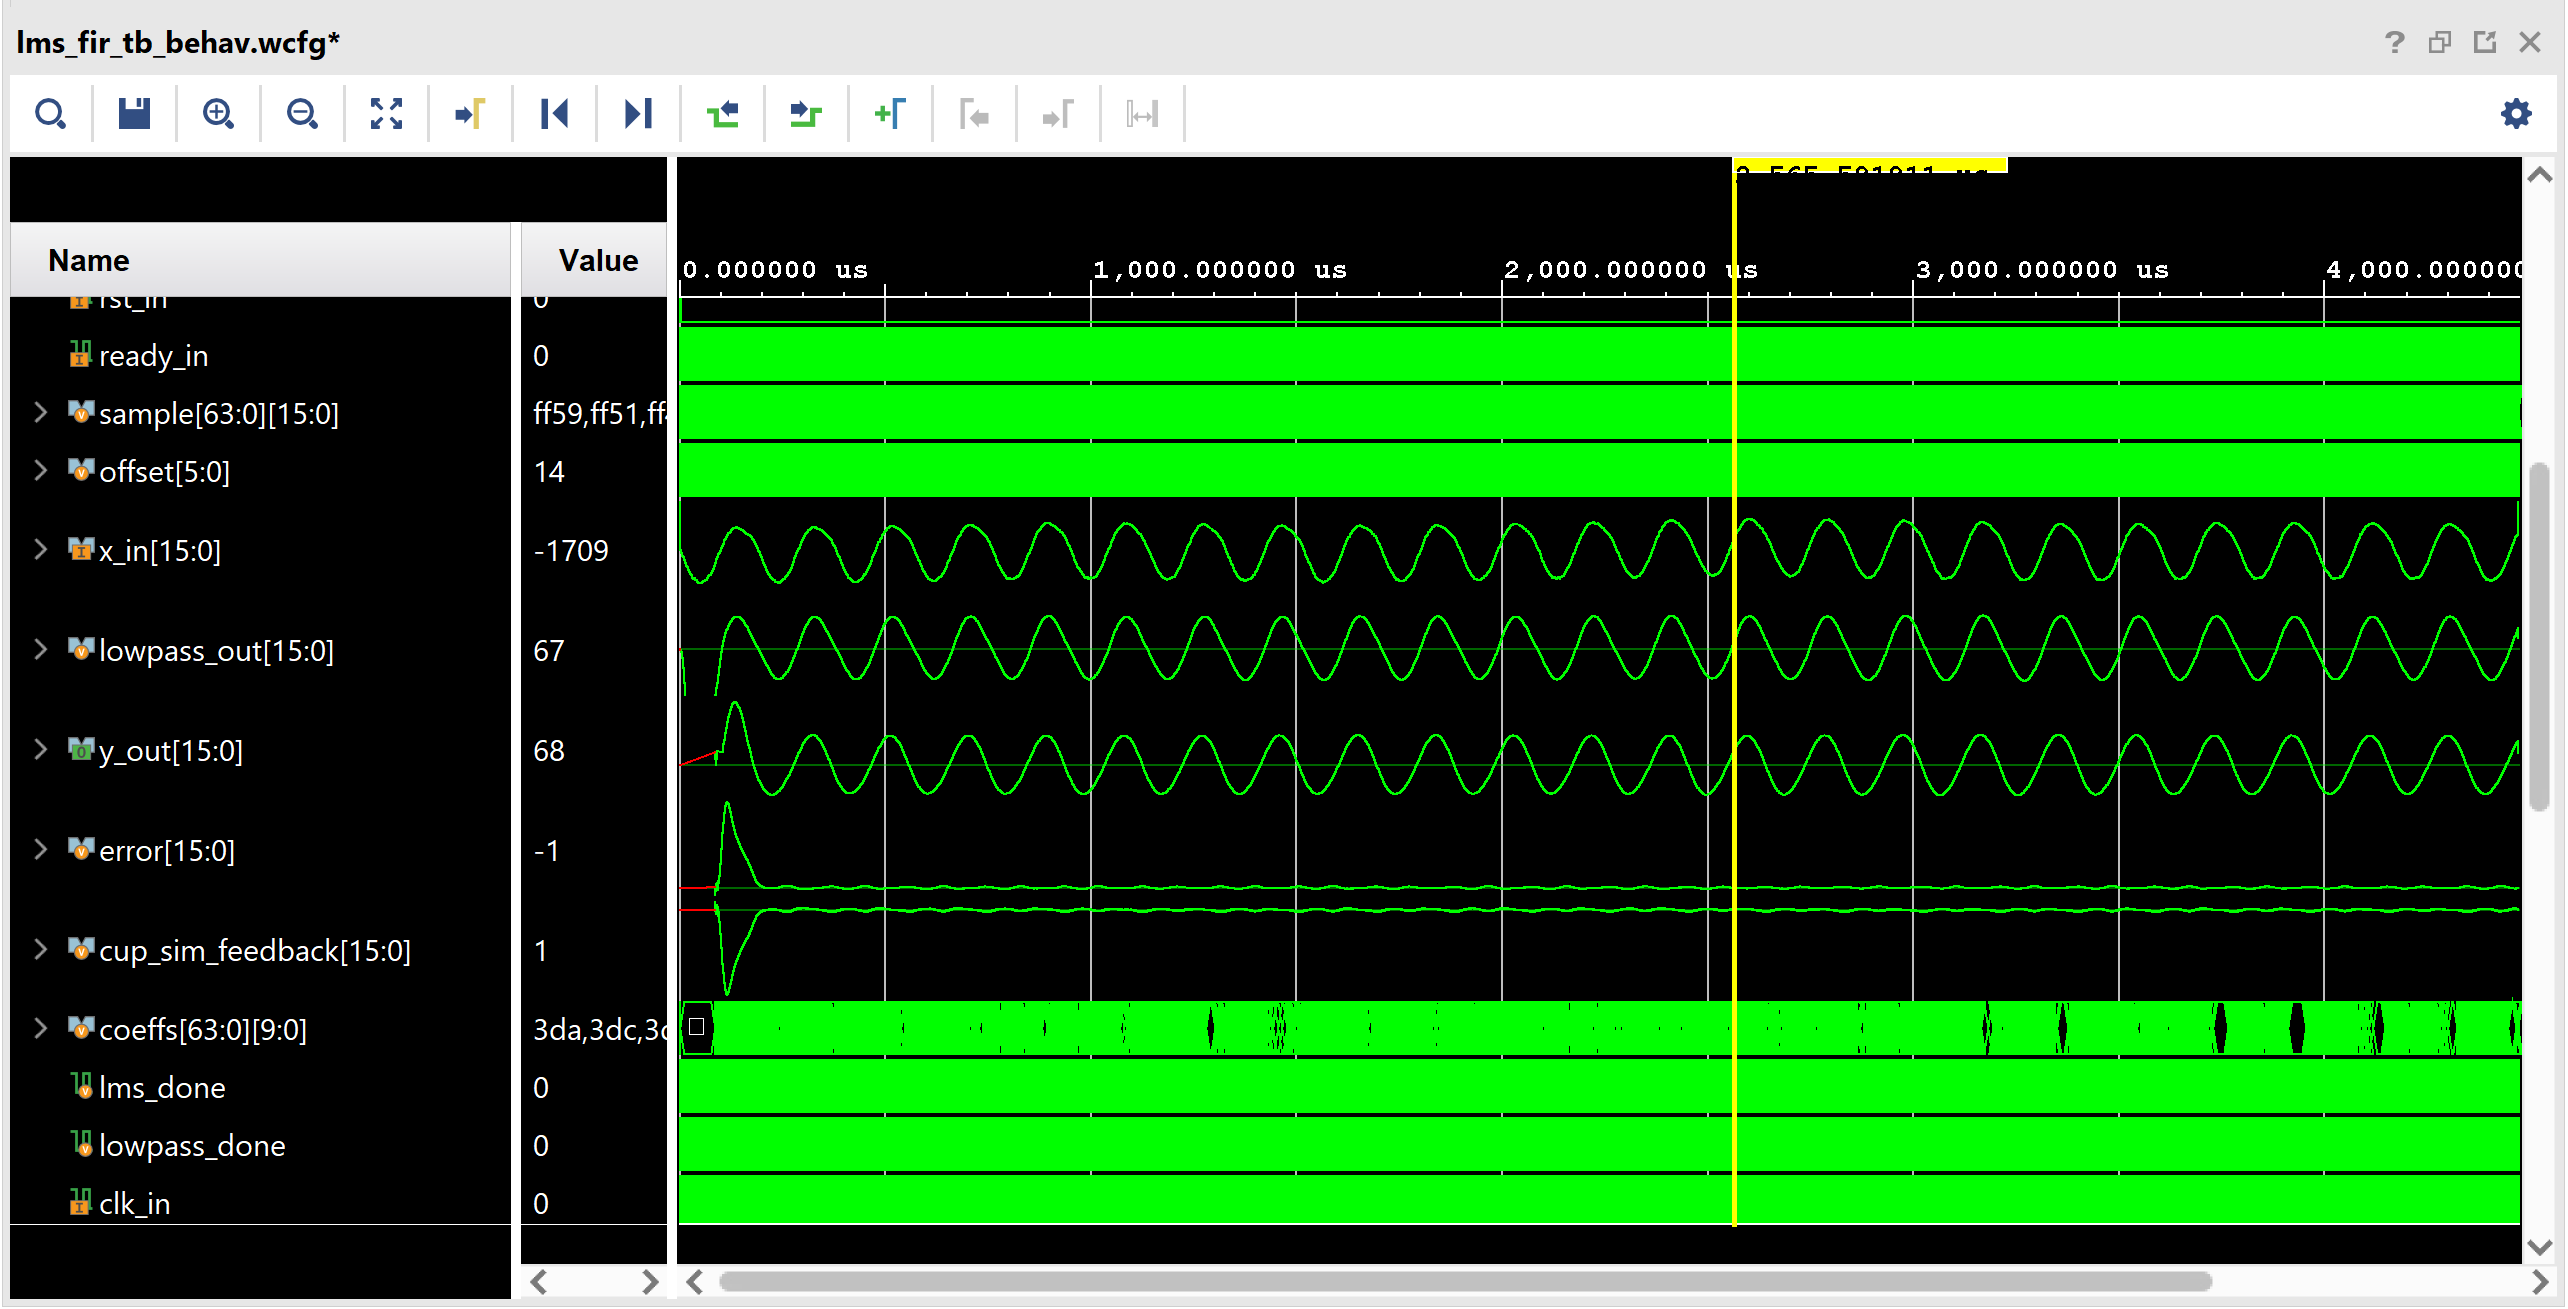
\includegraphics[width=450pt]{./figs/nlms_test_bench_sine_ila.png}
\caption{System converging on real sine tone noise (from ILA) in simulation}
\label{fig:sinenoisesimulation}

\bigskip
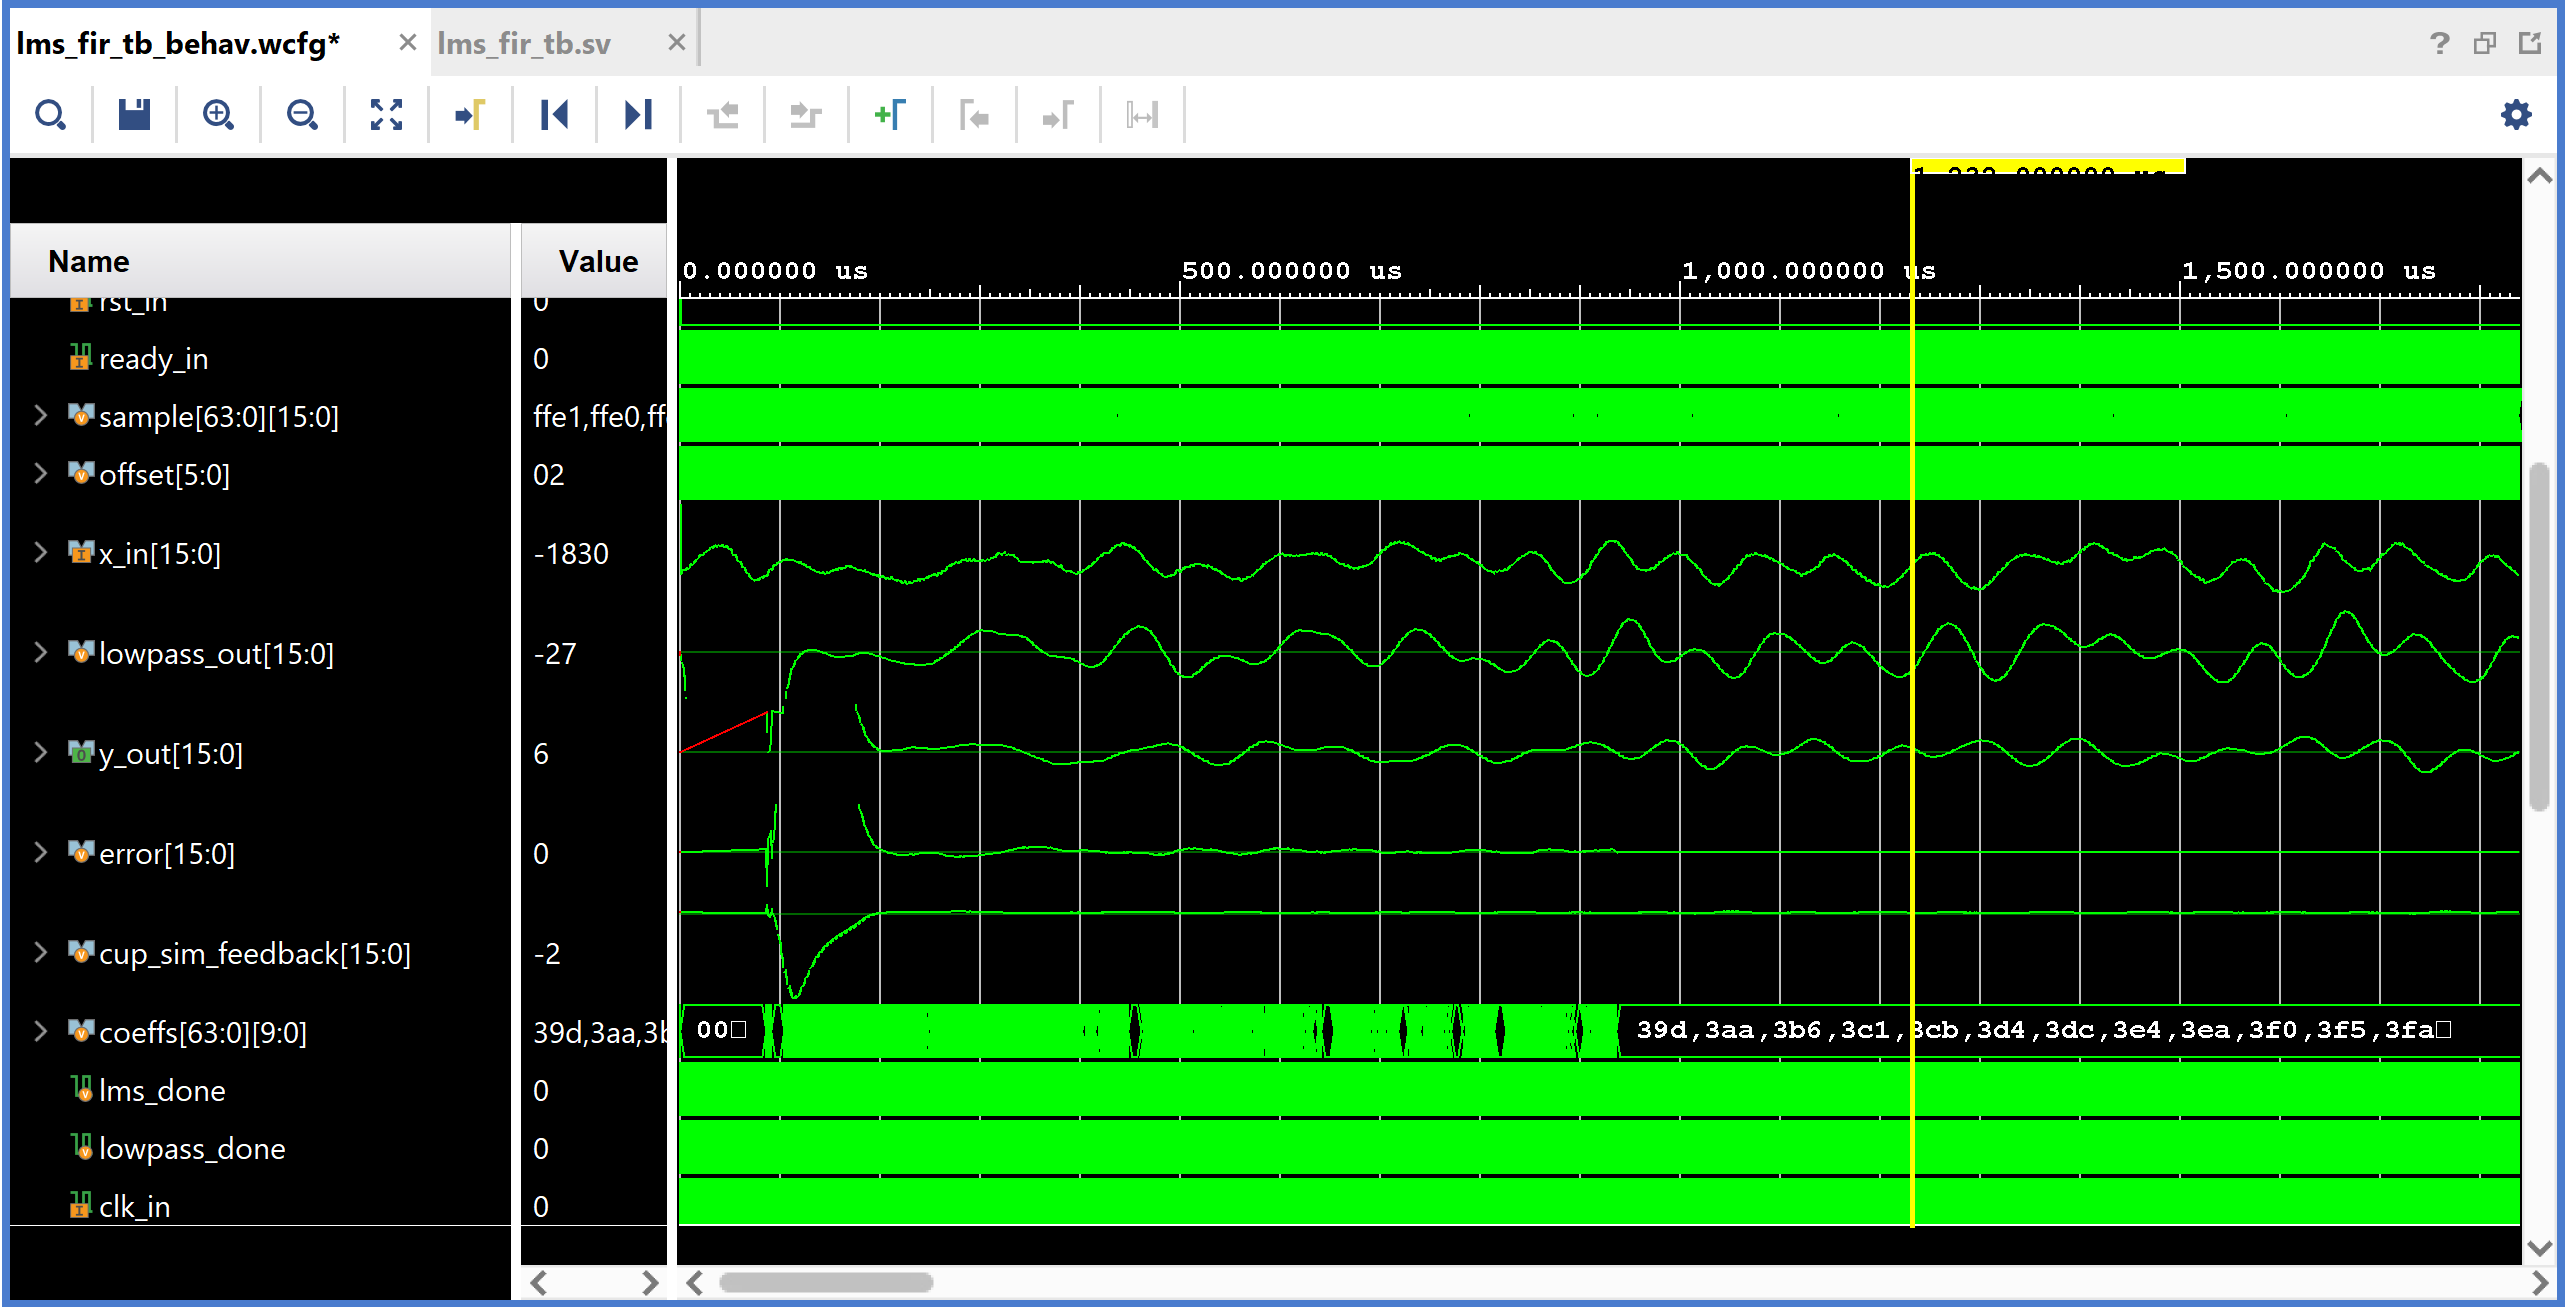
\includegraphics[width=450pt]{./figs/nlms_test_bench_plane_ila.png}
\caption{System converging on real ambient airplane noise (from ILA) in simulation}
\label{fig:ambientnoisesimulation}
\end{figure}

\section{Challenges}
\subsection{Feedback}
Our initial hardware testing setup did not include as much passive cancellation as our final design. In our initial trial, we immediately identified that this lack of passive cancellation, as well as a lack of materials to stop reflections, allowed the output of the speaker to be picked up by the ambient noise microphone, causing the system to become unstable. To resolve this, we added the additional enclosure described in the hardware section. This was designed both in order to stop reflections, absorbing them in the shipping foam, and to isolate the system from audio exiting or leaving the system from off-axis angles.

\subsection{Microphone Noise}
Our initial system picked up periodic spikes in the microphone inputs, which caused impulses on the speaker output. These impulses contributed even more to the feedback to the ambient noise microphone that caused our system to become unstable. We noticed that this happened on only one of the two microphones, and that if we switched the wiring to the two microphones, the error followed the wiring rather than the microphone itself. Perhaps unsurprisingly, this turned out to be a wiring or breadboarding issue, and simplifying the wiring to the two microphones removed this noise and gave a clean output from both microphones.

\subsection{Choosing LMS Step Size Empirically}
One of our initial ideas for the project was to implement the standard LMS algorithm which uses an empirically found step size. As mentioned above in the LMS and NLMS module explanations, finding a step size for LMS that enables convergence is very difficult. Our first step in trying to derive the correct step size was by implementing the LMS algorithm in python to get a better understanding of the algorithm and to make initial testing easier. Specifically, we tested this software version of LMS with sine tone waveforms to get a general range of possible step sizes that would allow LMS to converge. From the testing, we noticed LMS was only able to converge for really small step sizes such at $10^{-12}$, but it converged perfectly. We then implemented an HDL verision of LMS. We ran numerous simulations with differing step sizes on recorded ILA waveforms of sine tones playing. In general, the verilog simulations looked promising as the algorithm would minimize the coefficients correctly. However, running actual tests with our hardware test setup would lead to overall pretty bad results. We concluded that even though it is possible to choose a working step size, that step size does not apply well to differing inputs. Since LMS is sensitive to the size of the input, we ultimately decided to implement NLMS (which scales to the size of the input) instead.


\subsection{Instability of NLMS Convergence}
Once we had taken care of feedback in our physical system by constructing a more sound-isolating enclosure and optimized the speed of our LMS algorithm by modifying it to be normalized, we tested our system on a variety of different sine tones. We noticed that regardless of the tone, there was an almost periodic oscillation in amplitude within the feedback microphone signal. The size of this oscillation was quite significant, and from observing this pattern we derived that this seemed to be an issue in NLMS convergence. Essentially, the algorithm was able to converge and effectively cancel input sine tones, but would not maintain that convergence. We knew that if there was a way to hold our coefficients at a converged state, we could achieve long-term sine tone cancellation.

Thus, we modified our error calculator module to include a "locking" mechanism that allowed the system to stop coefficient updates once it recognized that it had achieved a desirable amount of cancellation. This is discussed in more detail within the description of our Error Calculator module earlier in the paper, but the general idea is that we set error to 0 once the feedback signal has settled within our target locking bounds, thus preventing the NLMS from changing any coefficients. This allowed us to achieve significant noise cancellation on sine tone inputs. Furthermore, we unlock coefficient updates by continuing to set the error to real values if the feedback signal has blown up past our target unlocking bounds. This allows the system to detect when the sine tone frequency being played has changed (this will make the feedback signal blow up, as the locked coefficients are no longer ideal for cancelling the new frequency). Thus, our system is able to re-converge and lock onto different sine tones automatically.

\subsection{Speaker Limitations}
In our testing, we noticed that the frequency response of our speaker was not flat, particularly at low frequencies. While our FIR coefficients were intended to cover this difference, we believe that they may have had insufficient resolution to accurately cover the wide range of frequency response of the speaker---this limitation of our system may have been one of the main reasons that we were unable to achieve our main goal of ambient noise cancellation---in the case of ambient noise, which is comprised of frequency content all over the spectrum, our system would have to encode the frequency response of our enclosure for a large number of frequencies. We quantified this by playing sine tones---all with constant amplitude---directly into the speaker, and using the signal measured by the feedback microphone to compare the speaker's response to each of these frequencies. Referring to the microphones datasheet, the microphone's frequency response is fairly flat in the range that we tested, so this difference must be due to the speaker itself. Figure \ref{chart:speaker_response} shows the result of this experimentation. Since this frequency response was so varied, especially in the 100-500Hz range that we were targeting, the number and resolution of our FIR coefficients may have limited our ability to encode this information. 

\begin{figure}
    \centering
    \begin{tikzpicture}
        \begin{axis}[
            title={Speaker Frequency Response},
            xlabel={Frequency Played (Hz)}, 
            ylabel={Difference from loudest frequency (dB)}
        ]
        \addplot table [
                x=f, 
                y=db, 
                col sep=comma, 
                scatter, 
                only marks 
            ] {charts/speaker_f_response.csv};
        \end{axis}
    \end{tikzpicture}
    \caption{Frequency response of the speaker used}
    \label{chart:speaker_response}
\end{figure}

\section{Reflections and Recommendations}
% perform benchmarking of system early in the process -- would have made us aware of the large difference in frequency response, I feel like we did not consider this as much as we should've

% invest in a testbench early on that is as accurate as possible. We got stuck waiting for parts, and having a better testbench would have helped us continue to make progress while waiting for parts and while constructing and debugging the physical system and its interfaces

% create a consistent interface for your modules, especially if they perform similar functions like our processing modules did. This allows much easier modification of the pipeline later to insert new modules, remove modules, or change the ordering. We added several modules over the course of our project, and if we had not done this, we would have had to rewrite modules to fit the new ones they were connected to.

Though we did not achieve our goal of effective ambient noise cancellation, we believe we implemented our base goal of sine tone cancellation very effectively, and we are proud of that. We learned about everything from signal processing to how physical systems behave and the many variables that we have to do our best to control when working with physical systems, and became much more familiar with FPGAs, their many uses, and the different mindset required to write HDL rather than software code. These differences were especially apparent in constructing our audio pipeline---we needed to ensure that each module finished before the next began, and also had some modules working in parallel. For example, our implementation included one chain working on feedback mic input, and one working on ambient mic input). Thinking about the timing and latency of different modules was crucial here to know which \ttt{done_out} signal would occur later and to ensure that we would be dealing with valid data and not have the pipelines out of sync. 

\appendix
\section{GitHub Repository}
We have used Git throughout the term for version control. Our code and supporting files are available in the repository at \url{https://github.com/bkettle/fpgairpods}.

\printbibliography

\end{document}
